\chapter{Digitalizing the Cube}
\myTop{In order to implement solving algorithms on a Rubik's Cube the cube itself must first be digitalized and a visual interface must be created in order to see the result of an algorithm. In this chapter that process is described.}
A \rubik{} is a rather simple three-dimensional structure, but implementing this structure into a computer system and getting it depicted on a two-dimensional screen is not a simple task.
The \rubik{} is build up by 26 moving \cpiece{}s held together by each other.  This type of structure is not straight forward to implement into a computer, so a way to handle these \cpiece{}s is needed.

%If the \rubik{} is depicted in the computer in a two-dimensional space, its depiction will be far from the original \rubik{} structure.
A simple way to handle the \rubik{} in the program is a two-dimensional depiction and  just simply move the \facelet{}s around.
The analogue to this on a real \rubik{} would be to take of the colored stickers off and move them to their new position rather than actually move the \cubie{}s when twisting the \rubik{}.
This approach will be far from reality and will make the implementations of solving algorithms, such as Kociemba's optimal solver and the beginner's algorithm more complicated, since they need to know the place of the \cpiece{}s, and not just the \facelet{}s to determine the next step.

A more object-oriented approach than to move the sticker would give a more useful structure for solving the problem.
If we divided the \rubik{} into it's sub structures it consists of six faces each with nine shared \cubie{}s.
%Dividing the \rubik{} into its sub structures. 
%The cube consist of the 6 faces each with 9 shared \cpiece{}. 
A face also consists of nine \cubicle{}s which act as placeholders for the \cpiece{}s. 
There are three types of \cpiece{}s and \cubicle{}s; corner, edge and centers. 
The center \cpiece{}s will never move and therefore there are no reason to define a \cubicle{} and a \cpiece{} for those. Instead the face is simple granted a \facelet{} which defines the color of the given face.
There are three types of \cpiece{}s and \cubicle{}s; corner, edge and centers. 
The center \cpiece{}s will never move and therefore there are no reason to define a \cubicle{} and a \cpiece{} for those. Instead the face is simple granted a \facelet{} which defines the color of the given face.
There are three types of \cpiece{}s and \cubicle{}s: corners, edges, and centers. 
The center \cpiece{}s will never move and therefore there is no reason to define a \cubicle{} and a \cpiece{} for those. Instead the center piece of a face is granted a colored \facelet{}, which defines the color of the face in the completed state of the \rubik{}.
\begin{figure}[h]
	\centering
		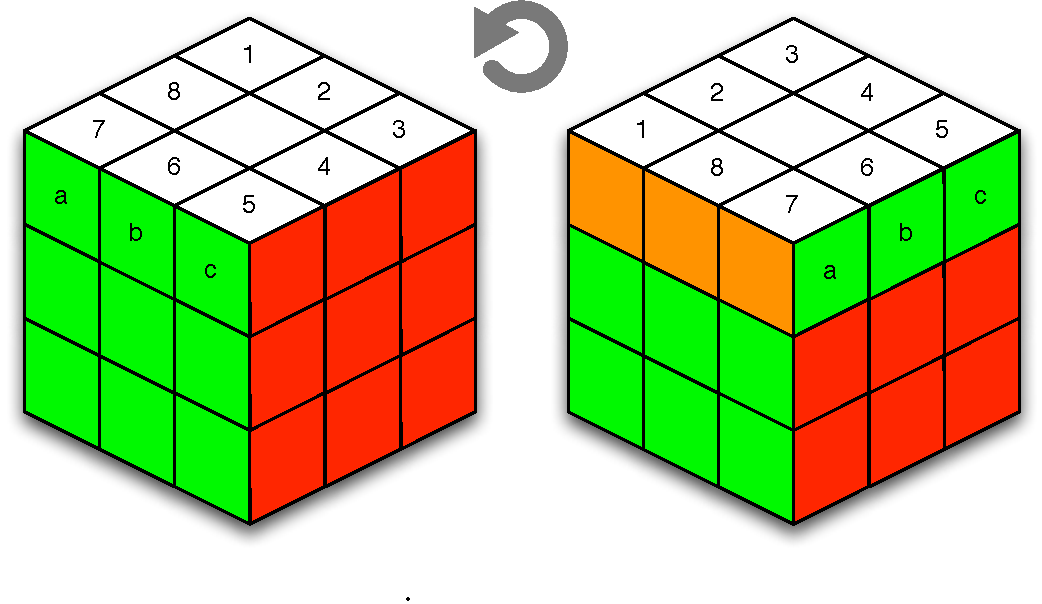
\includegraphics[scale=0.6]{input/pics/twistOfUpFace.pdf}
	\caption{\myCaption{A twist of a face will not only inflict the twisted face but also its adjacent faces. }}
	\label{fig:twistOfUpFace}
\end{figure}
This structure allows for the same \cubicle{} to be in several faces -- two faces for edges and three for corners. 
In this structure moving a \face{} will move the \cpiece{}s from one \cubicle{} to another. See figure \ref{fig:twistOfUpFace}. By performing a \twist{} the \face{}s adjacent to the twisted \face{} are also affected. 
For example when \twist{}ing the up face of a \rubik{} the \cubie{}s adjecent to the up face in R, L, B, and F faces will be permuted.

However the problem of this structure is that it requires variables to determine how the \cubie{}s are oriented. 
How this is done is described in the next section ref\{Somewhere\}.
